\begin{figure}[htbp]
  \begin{tabular}{cc}
    \begin{minipage}{0.5\hsize}
      \centering
      \includegraphics[width=6.0cm]{../pic/Dron/comp_kamano_I0.eps}
    \end{minipage}

    \begin{minipage}{0.5\hsize}
      \centering
      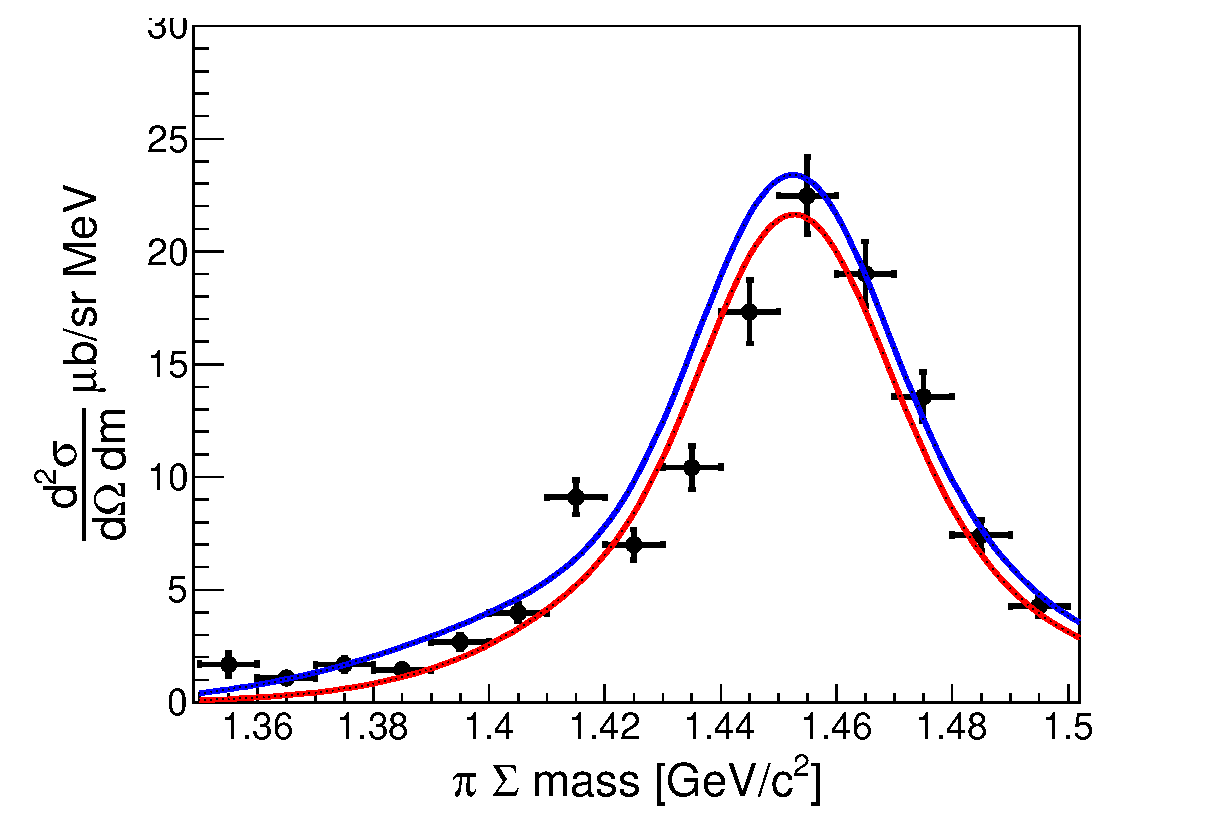
\includegraphics[width=6.0cm]{../pic/Dron/comp_kamano_interfer.eps}
    \end{minipage}
  \end{tabular}

  \centering
  \includegraphics[width=6.0cm]{../pic/Dron/comp_kamano_I1.eps}
  \caption{
    These figures show a comparison between our data and theoretical calculations of the DCC models (models.A and model.B).
    The black error bars represent our data.
    The blue and red lines represent Model.A and Model.B respectively.
    The top right figure shows the strength of $I=0$, the top left figure shows the interference term and the bottom figure shows the strength of $I=1$.
  }
  \label{fig:decomposed_DCC}
\end{figure}
